\documentclass[12pt]{article}
\usepackage[utf8]{inputenc}
\usepackage{float}
\usepackage{amsmath}

\usepackage{tikz}
\usepackage[hmargin=3cm,vmargin=6.0cm]{geometry}
\topmargin=-2cm
\addtolength{\textheight}{6.5cm}
\addtolength{\textwidth}{2.0cm}
\setlength{\oddsidemargin}{0.0cm}
\setlength{\evensidemargin}{0.0cm}
\usepackage{indentfirst}
\usepackage{amsfonts}

\usepackage{listings}

\begin{document}

\subsection*{c)} 



\begin{lstlisting}
GE_70 = 0;
GE_85 = 0;

for i = 1:1000		
    sample = normrnd(65, 6, 100, 1);
    total = sum(sample > 60 & sample < 75);	
    
    if total >= 70
        GE_70 += 1;
    end
    if total >= 85
        GE_85 += 1;
    end
end

GE_70
GE_85

\end{lstlisting}

\[ \text{ GE 70: at least 70 percent of the elephants had a lifespan in the given range } \]

\[ \text{ GE 85: at least 85 percent of the elephants had a lifespan in the given range } \]

\begin{figure}
  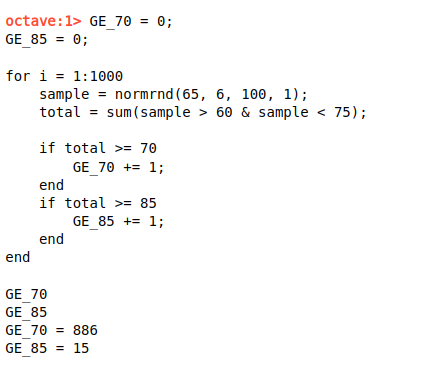
\includegraphics[width=\linewidth]{4c.png}
  \label{4c}
\end{figure}





\end{document}
